\documentclass[10pt,letterpaper]{article}

\usepackage[margin=0.70in]{geometry}
\usepackage[T1]{fontenc}
\usepackage{lmodern}
\usepackage{microtype}
\usepackage{graphicx}
\usepackage{booktabs}
\usepackage{tabularx}
\usepackage{longtable}
\usepackage{array}
\usepackage{enumitem}
\usepackage{fancyhdr}
\usepackage{hyperref}
\usepackage{pdflscape}
\usepackage{xcolor}
\usepackage{listings}
\usepackage{amsmath,amssymb}
\usepackage{titlesec}
\usepackage{caption}
\usepackage{lastpage}

\hypersetup{colorlinks=true,linkcolor=black,urlcolor=black,citecolor=black,pdfauthor={Komorebi P.},pdftitle={PRISM-1R Implementation and Deployment Blueprint v0.2}}

\definecolor{RuleGray}{gray}{0.35}
\definecolor{LightGray}{gray}{0.94}
\definecolor{MidGray}{gray}{0.82}
\definecolor{DarkGray}{gray}{0.18}

\pagestyle{fancy}
\fancyhf{}
\lhead{\small KOMOREBI PRISM-1R}
\rhead{\small Implementation and Deployment Blueprint v0.2}
\cfoot{\small \thepage}
\renewcommand{\headrulewidth}{0.4pt}

\titleformat{\section}{\Large\bfseries}{\thesection.}{0.6em}{}
\titleformat{\subsection}{\large\bfseries}{\thesubsection}{0.5em}{}
\titleformat{\subsubsection}{\normalsize\bfseries}{\thesubsubsection}{0.45em}{}
\setlist[itemize]{leftmargin=1.25em,itemsep=2pt,topsep=3pt}
\setlist[enumerate]{leftmargin=1.35em,itemsep=2pt,topsep=3pt}
\setlength{\parindent}{0pt}
\setlength{\parskip}{5pt}
\renewcommand{\arraystretch}{1.16}

\newcommand{\statusbox}[2]{%
  \vspace{3pt}\noindent\fbox{\begin{minipage}{0.96\linewidth}\textbf{#1}\quad #2\end{minipage}}\vspace{3pt}%
}
\newcommand{\code}[1]{\texttt{#1}}
\newcommand{\good}{\textbf{PASS}}
\newcommand{\stopgate}{\textbf{STOP}}

\lstset{
  basicstyle=\ttfamily\footnotesize,
  backgroundcolor=\color{LightGray},
  frame=single,
  rulecolor=\color{MidGray},
  breaklines=true,
  columns=fullflexible,
  showstringspaces=false,
  xleftmargin=2mm,
  xrightmargin=2mm
}

\begin{document}

% -----------------------------------------------------------------------------
% COVER
% -----------------------------------------------------------------------------
\thispagestyle{empty}
\vspace*{0.55in}
\begin{center}
{\Huge\bfseries PRISM-1R}\\[0.12in]
{\LARGE\bfseries Implementation and Deployment Blueprint v0.2}\\[0.18in]
{\large Packet-programmable mixed-representation accelerator}\\[0.05in]
{\large Transformation plane + resolution plane + certificate-gated commit}\\[0.45in]

\rule{0.90\linewidth}{0.8pt}\\[0.28in]

\begin{tabularx}{0.88\linewidth}{>{\bfseries}p{1.55in}X}
Baseline & PRISM-1 Final Updated architecture specification \\
Revision & PRISM-1R physicalization and deployment blueprint \\
Deployment target & Golden model $\rightarrow$ CUDA $\rightarrow$ cycle simulator $\rightarrow$ FPGA $\rightarrow$ shuttle chiplet $\rightarrow$ reference chiplet $\rightarrow$ full package \\
Primary rule & Preserve structure. Execute locally. Refine only where evidence requires it. \\
Status & Engineering blueprint. Not fabricated silicon. All frequency, bandwidth, area and power values remain design targets until measured. \\
\end{tabularx}

\vfill
{\large Komorebi P.}\par
\vspace{0.08in}
{\small Implementation handoff draft v0.2}\par
\end{center}
\newpage

\tableofcontents
\newpage

% -----------------------------------------------------------------------------
\section{Purpose and Deployment Philosophy}

PRISM-1R converts the existing PRISM architecture into an implementation program. The objective is not to freeze every circuit choice prematurely. The objective is to freeze the \emph{semantic contracts} that software, simulation, FPGA and ASIC implementations must share, while keeping physical parameters adjustable until measurement and synthesis justify them.

The architecture is organized around one principle:
\[
\boxed{\text{Do not materialize, move, or schedule structure already declared inactive.}}
\]

PRISM-1R adds a second principle:
\[
\boxed{\text{Do not execute at a resolution that current evidence has already invalidated.}}
\]

The machine therefore chooses four quantities jointly:
\[
\boxed{(\text{representation},\ \text{resolution},\ \text{placement},\ \text{precision}).}
\]

A dense tensor remains a legal representation and fallback. It is not privileged as mandatory machine state.

\statusbox{Scope boundary.}{This document specifies interfaces, resource organization, deployment stages, verification obligations, prototype gates, and operating procedures. It does not claim completed production RTL, timing closure, physical signoff, fabricated silicon performance, or measured package power.}

% -----------------------------------------------------------------------------
\section{Reference Configuration}

The reference package preserves the broad PRISM-1 scale while revising locality and control organization.

\begin{table}[h]
\centering
\caption{PRISM-1R reference targets. Values are design targets, not measured silicon.}
\begin{tabularx}{0.96\linewidth}{Xr}
\toprule
\textbf{Resource} & \textbf{Reference target}\\
\midrule
Compute chiplets & 4\\
Packet Streaming Multiprocessors (PSMs) & 64 total\\
PSMs per chiplet & 16\\
Quadrants per chiplet & 4\\
Execution groups & 256 total\\
Execution groups per PSM & 4\\
Matrix array per execution group & $16\times16$\\
Clock modeling point & 1.5 GHz\\
Scratchpad per PSM & 2 MiB\\
Physical scratchpad banks & 16 $\times$ 128 KiB\\
Shared SRAM per chiplet & 16 MiB\\
Total local + shared SRAM & 192 MiB\\
Transform engines & 32 total\\
Small-solver engines & 16 total\\
Exact arithmetic clusters & 4 total\\
HBM4 stacks & 4\\
Reference HBM capacity & 144 GiB total\\
Reference aggregate HBM bandwidth & $>11.2$ TB/s\\
Package link class & UCIe 3.0 class\\
Host link class & PCIe 7.0 x16 class, optional CXL\\
Reference package power envelope & 500 W\\
\bottomrule
\end{tabularx}
\end{table}

Dense peak remains secondary. The architecture succeeds only when mathematical structure removes enough arithmetic, storage, synchronization, or movement to justify specialized execution.

% -----------------------------------------------------------------------------
\section{Python-Generated Architecture Blueprint}

The following blueprint is generated programmatically from the same reference parameters used by this deployment guide. The figure is intended to function as an implementation map rather than a presentation illustration.

\begin{landscape}
\thispagestyle{empty}
\begin{center}
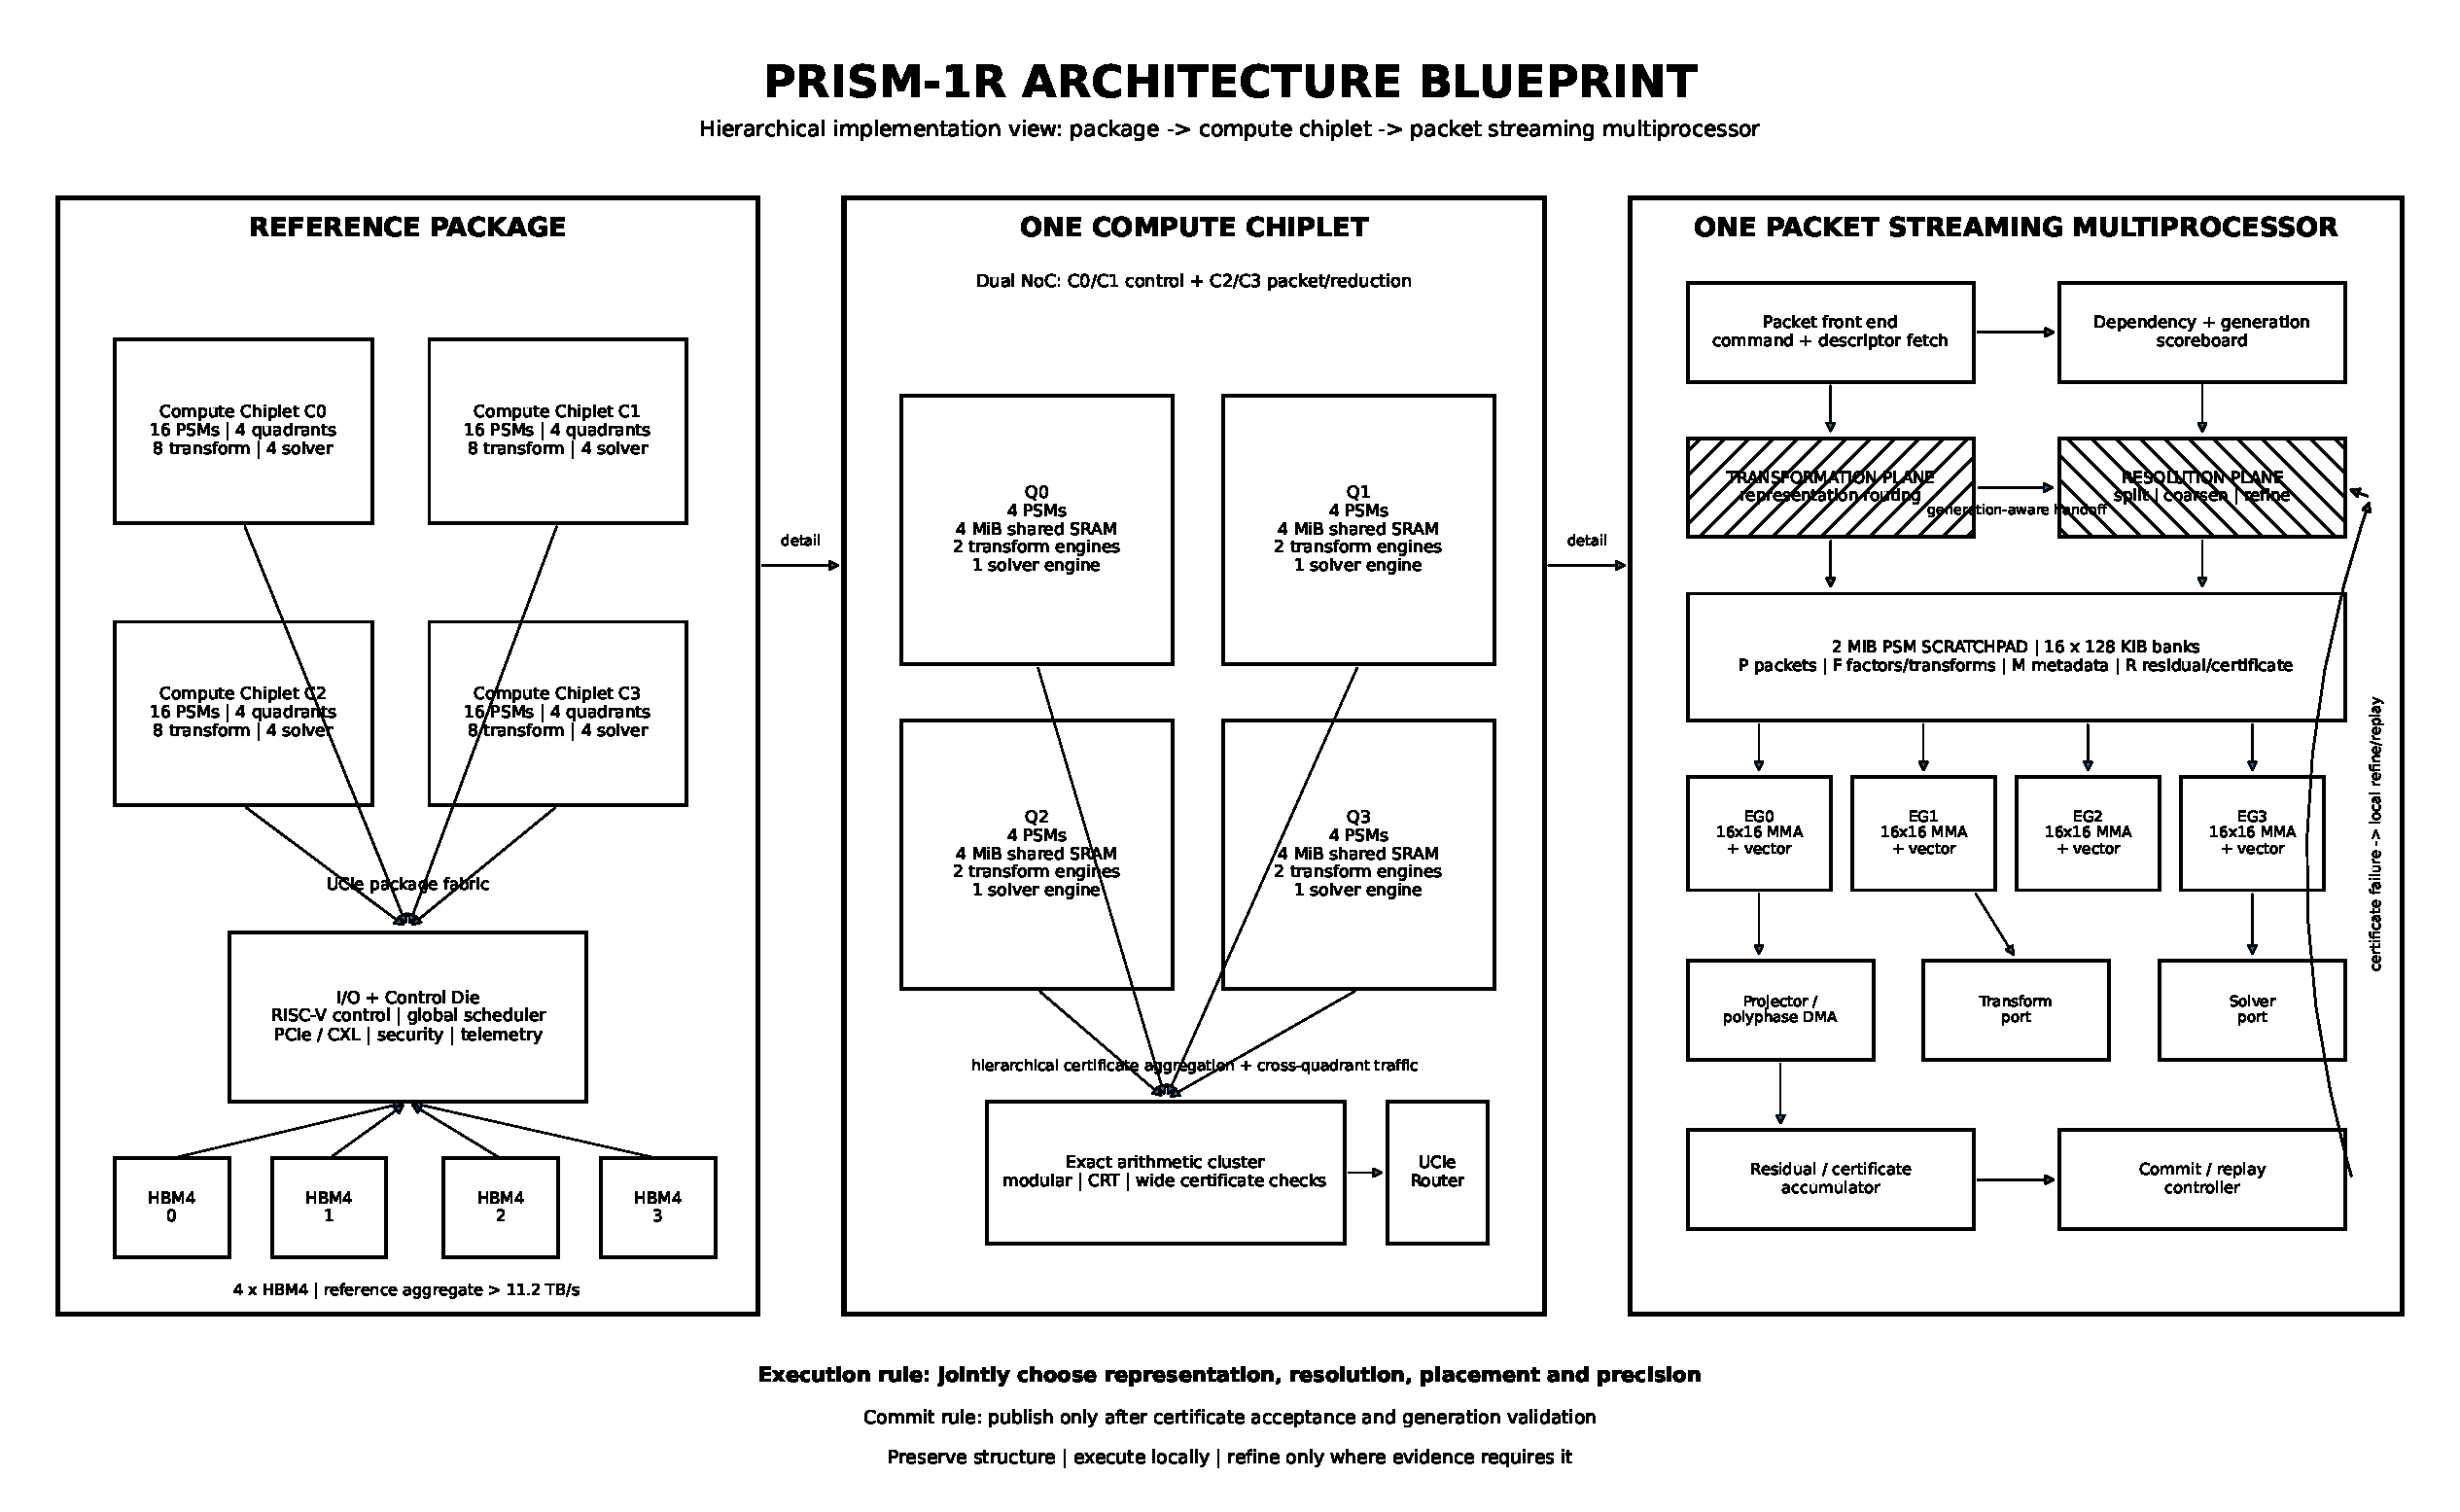
\includegraphics[width=0.985\linewidth]{../figures/PRISM-1R_Python_Architecture_Blueprint.pdf}
\end{center}
\end{landscape}

% -----------------------------------------------------------------------------
\section{What Must Be Frozen Before Production RTL}

Freeze semantics before circuit details. A production RTL effort should not begin until the following objects have versioned, testable definitions.

\begin{enumerate}
\item Packet descriptor semantics.
\item Transfer-edge descriptor semantics.
\item Atlas and selector semantics.
\item Refinement-family and parent/child semantics.
\item Representation and output-contract semantics.
\item Dependency token and completion token semantics.
\item Generation-number invalidation semantics.
\item Precision, sensitivity, and error-budget semantics.
\item Certificate acceptance semantics.
\item Commit, replay, and fault-containment semantics.
\item Command-buffer ABI and completion-record ABI.
\item Packet IR canonical serialization.
\item CUDA/PRISM backend conformance requirements.
\end{enumerate}

The following should remain parameterized until synthesis, FPGA measurement, or floorplanning provides evidence: scratchpad port width, final SRAM macro organization, issue width, exact NoC link width, number of virtual channels beyond the minimum classes, DVFS domains, exact root-solver microarchitecture, and hardened interface IP choices.

% -----------------------------------------------------------------------------
\section{Dual-Plane Execution Model}

PRISM-1R separates two control problems that were previously too implicit.

\subsection{Transformation plane}

The transformation plane performs computation within the current representation and resolution:
\[
P_\alpha x \longmapsto P_\beta T P_\alpha x.
\]

Typical operations include block matrix products, low-rank contractions, transform stages, Kronecker mode products, sparse-chain applications, modular operations, nonlinear memory kernels, reductions, and small solves.

\subsection{Resolution plane}

The resolution plane modifies the decomposition itself:
\[
P_\alpha \longleftrightarrow \{P_{\alpha_1},\ldots,P_{\alpha_k}\}.
\]

It handles split, coarsen, local refinement, atlas changes, reconstruction changes, and replay boundaries.

\subsection{Generation guard}

Each mutable packet family carries a generation number $g$. A command records the generation it consumed. Refinement increments $g$ for the affected family. A provisional result may commit only if
\[
\boxed{g_{\rm consumed}=g_{\rm current}.}
\]

This mechanism converts stale work after adaptive refinement into an explicit hardware predicate rather than a software convention.

% -----------------------------------------------------------------------------
\section{Packet Streaming Multiprocessor Blueprint}

One PSM is the independently scheduled execution unit. The recommended block composition is:

\begin{lstlisting}
Packet front end
  -> dependency / generation scoreboard
  -> representation router -----------+
  -> resolution controller -----------|--- adaptive control
                                      |
16-bank 2 MiB scratchpad <------------+
  -> EG0: 16x16 MMA + vector
  -> EG1: 16x16 MMA + vector
  -> EG2: 16x16 MMA + vector
  -> EG3: 16x16 MMA + vector
  -> projector / polyphase DMA
  -> transform port
  -> solver port
  -> local reduction fabric
  -> residual / certificate accumulator
  -> commit / replay controller
\end{lstlisting}

\begin{figure}[ht]
\centering
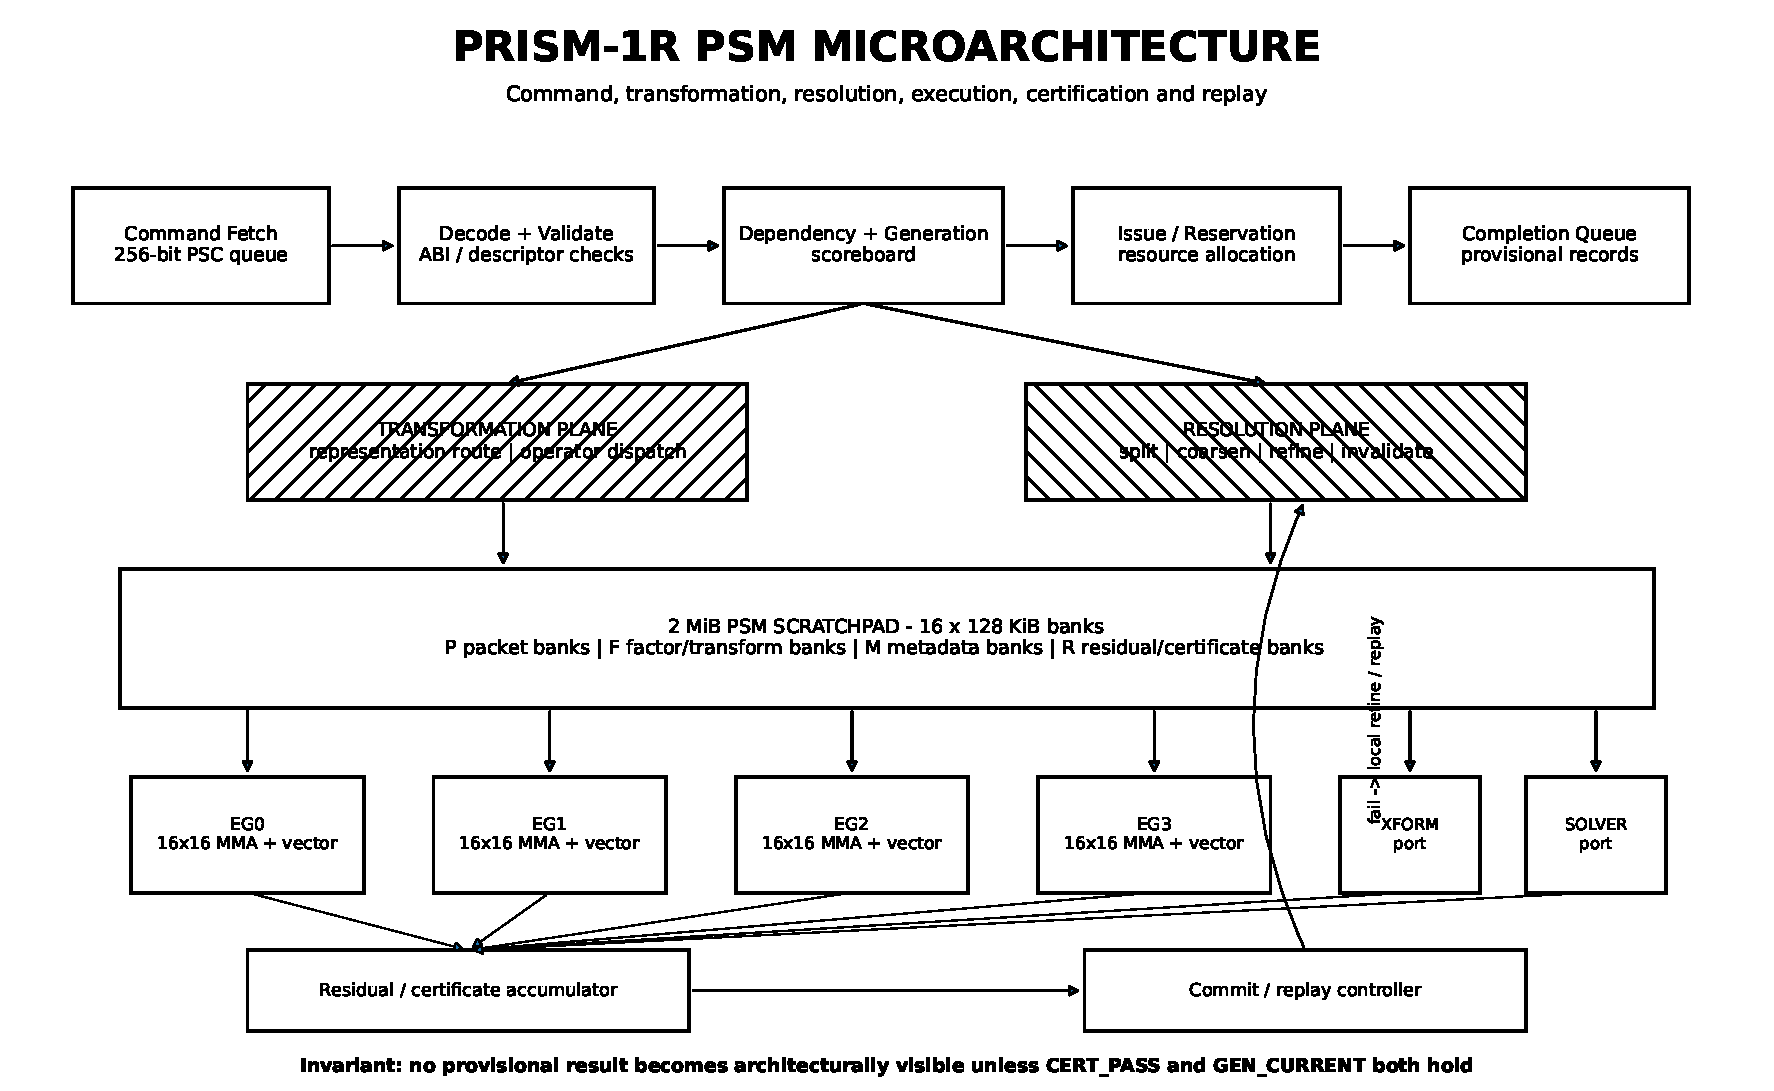
\includegraphics[width=0.98\linewidth]{../figures/02_psm_microarchitecture.pdf}
\caption{Implementation-oriented PSM microarchitecture. The transformation plane executes within the current decomposition; the resolution plane changes that decomposition and can trigger bounded replay.}
\end{figure}

Each execution group is intentionally modest. The PSM is not designed to maximize unstructured GEMM density. It is designed to keep the selected representation resident and avoid repeated conversion into a generic dense form.

\subsection{Command state machine}

A minimal command lifecycle is
\[
\texttt{QUEUED}
\rightarrow \texttt{READY}
\rightarrow \texttt{DISPATCHED}
\rightarrow \texttt{PROVISIONAL}
\rightarrow \texttt{CERTIFIED}
\rightarrow \texttt{COMMITTED}.
\]

Failure paths are explicit:
\[
\texttt{PROVISIONAL}\rightarrow \texttt{REFINE}\rightarrow\texttt{REPLAY}
\]
or
\[
\texttt{PROVISIONAL}\rightarrow \texttt{ABORT}.
\]

Kernel completion and architectural visibility are therefore different events.

% -----------------------------------------------------------------------------
\section{Scratchpad and Memory System}

\subsection{PSM scratchpad}

Keep the 2 MiB capacity but replace the vague four-bank concept with 16 physical banks:
\[
16\times128\text{ KiB}=2\text{ MiB}.
\]

Retain four logical allocator classes:

\begin{table}[h]
\centering
\begin{tabularx}{0.94\linewidth}{>{\bfseries}p{0.55in}p{1.6in}X}
\toprule
Class & Name & Typical contents\\
\midrule
P & Packet region & active blocks, packet outputs, local destination accumulators\\
F & Factor region & low-rank factors, transform stages, Kronecker factors, solver panels\\
M & Metadata region & descriptors, selectors, indices, dependency state, compact graph records\\
R & Residual region & residuals, norms, certificate state, replay records, refinement summaries\\
\bottomrule
\end{tabularx}
\end{table}

The classes are compiler-visible pools, not rigid physical partitions.

\subsection{Bandwidth modeling point}

If each of 16 banks supplies a 256-bit word per cycle, the aggregate raw bandwidth is
\[
16\times 32\text{ B/cycle}=512\text{ B/cycle}.
\]
At 1.5 GHz this is
\[
\boxed{768\text{ GB/s per PSM raw scratchpad bandwidth}.}
\]

A simple FP16 feed estimate for one $16\times16$ array is 32 FP16 operands per active cycle, or 64 B/cycle. Four execution groups therefore require roughly
\[
4\times64=256\text{ B/cycle}
\]
for direct operand feed before output traffic and reuse effects, corresponding to approximately 384 GB/s at 1.5 GHz. The proposed bank organization therefore begins with roughly 2x raw headroom against that simplified feed estimate. This is a modeling target, not a timing guarantee.

\subsection{Hierarchy}

\begin{itemize}
\item HBM: exact archive, cold factors, large graphs, model history, oversized packets.
\item Chiplet shared SRAM: active packet graph, hot immutable factors, cross-PSM transform state.
\item PSM scratchpad: active tiles, factors, solver panels, residuals, local metadata.
\item Registers / array state: immediate execution state.
\end{itemize}

% -----------------------------------------------------------------------------
\section{Chiplet Quadrant Organization}

A compute chiplet is divided into four locality quadrants. Each quadrant contains:
\[
\boxed{4\text{ PSMs}+4\text{ MiB shared SRAM}+2\text{ transform engines}+1\text{ solver}.}
\]

This exactly consumes the chiplet-level reference resources while reducing the distance between packet execution, transform stages, and small solves.

The placement objective is not merely minimum latency. It is minimum structured movement:
\[
\min \sum_{e\in E} \operatorname{bytes}(e)\times\operatorname{hops}(e).
\]

Hot factors should be replicated read-only where the replication cost is lower than repeated network movement. Mutable packet state should retain clear ownership.

% -----------------------------------------------------------------------------
\section{Network-on-Chip Blueprint}

PRISM-1R uses separate logical control and payload service, even if an implementation shares physical wires.

\begin{table}[h]
\centering
\caption{Minimum traffic classes.}
\begin{tabularx}{0.97\linewidth}{p{0.55in}p{1.55in}X X}
\toprule
\textbf{Class} & \textbf{Traffic} & \textbf{Service rule} & \textbf{Examples}\\
\midrule
C0 & commit / fault & forward-progress guaranteed & certificate acceptance, dependency wakeup, invalidation, exception\\
C1 & metadata & latency-oriented & descriptors, compact graph state, selector records\\
C2 & payload & bandwidth-oriented & blocks, factors, transform streams, packet transfers\\
C3 & reduction & bounded service & residual summaries, tree reductions, reconstruction contributions\\
\bottomrule
\end{tabularx}
\end{table}

C2 saturation must never prevent C0 progress. This is a correctness requirement, not only a performance preference.

\begin{figure}[ht]
\centering
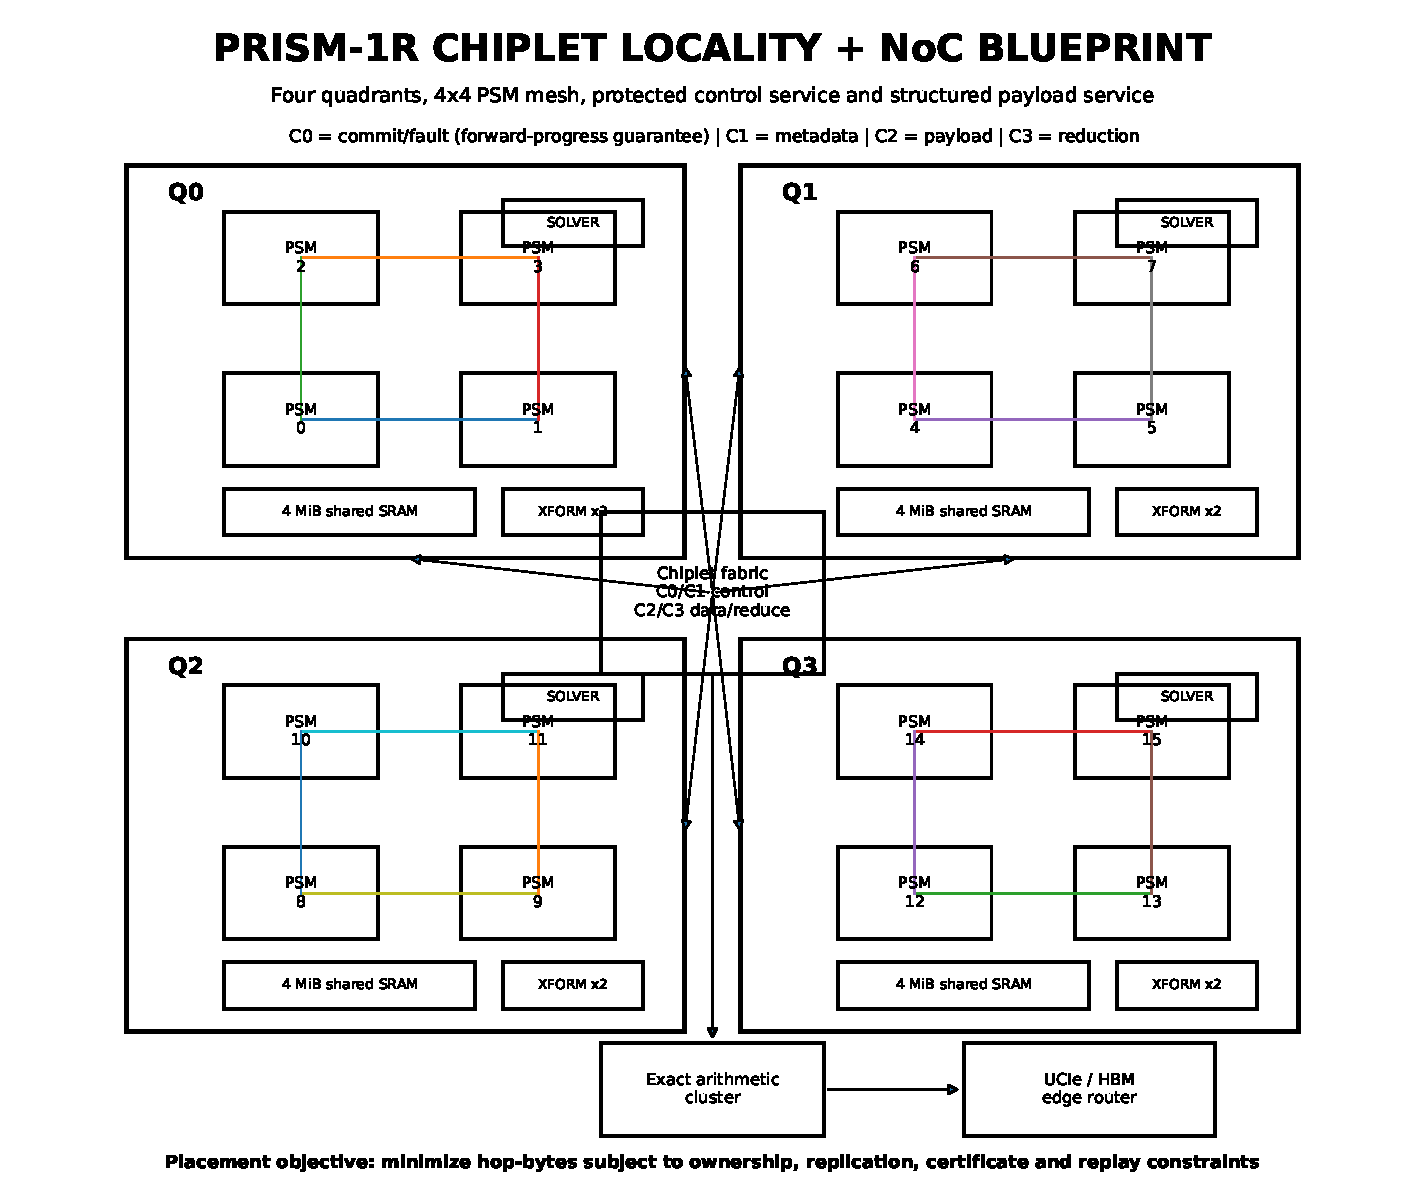
\includegraphics[width=0.91\linewidth]{../figures/03_chiplet_noc_locality.pdf}
\caption{Chiplet locality and NoC organization. Quadrant locality is the default placement unit, while cross-quadrant traffic remains explicit and measurable.}
\end{figure}

An initial packet-link modeling point is 1024 bits at 1.5 GHz:
\[
128\text{ B/cycle}\times1.5\text{ GHz}=\boxed{192\text{ GB/s per unidirectional link}}
\]
before encoding, arbitration, flow control, ECC, and protocol overhead.

\subsection{Residency states}

Avoid a CPU-style general coherence protocol. Use three architectural residency states:

\begin{description}[leftmargin=1.25in,style=nextline]
\item[owned] one location may mutate the packet or representation state;
\item[replicated-read] immutable factors, atlas data, or descriptors may exist at multiple locations;
\item[streaming] the payload has no persistent residency and is consumed in flight.
\end{description}

Generation invalidation handles stale read replicas associated with refinement.

% -----------------------------------------------------------------------------
\section{Certificate, Commit, and Replay}

Certification is a first-class data path. A kernel result is provisional until its declared acceptance rule passes.

\subsection{Fused accumulation}

Do not implement certification as a second full read of the result. Execution should tap quantities such as residual components, norms, energy partitions, trace summaries, rank margins, rounding bounds, and branch margins while the producing data is already live.

\subsection{Hierarchical aggregation}

Use the hierarchy
\[
\text{execution group}\rightarrow\text{PSM}\rightarrow\text{quadrant}\rightarrow\text{chiplet}\rightarrow\text{exact cluster when required}.
\]

For example, local squared residual summaries may reduce as
\[
R_P^2=\sum_i r_i^2
\]
without transmitting the original packet tensor through the certificate network.

\subsection{Commit predicate}

A provisional result commits only if all required conditions hold:
\[
\boxed{
\texttt{CERT\_PASS}
\land
\texttt{GEN\_CURRENT}
\land
\texttt{NO\_UNCORRECTABLE\_FAULT}
\land
\texttt{DEPENDENCIES\_VALID}.
}
\]

A failure should invalidate the smallest declared replay region unless the error is explicitly package-wide.

\begin{figure}[ht]
\centering
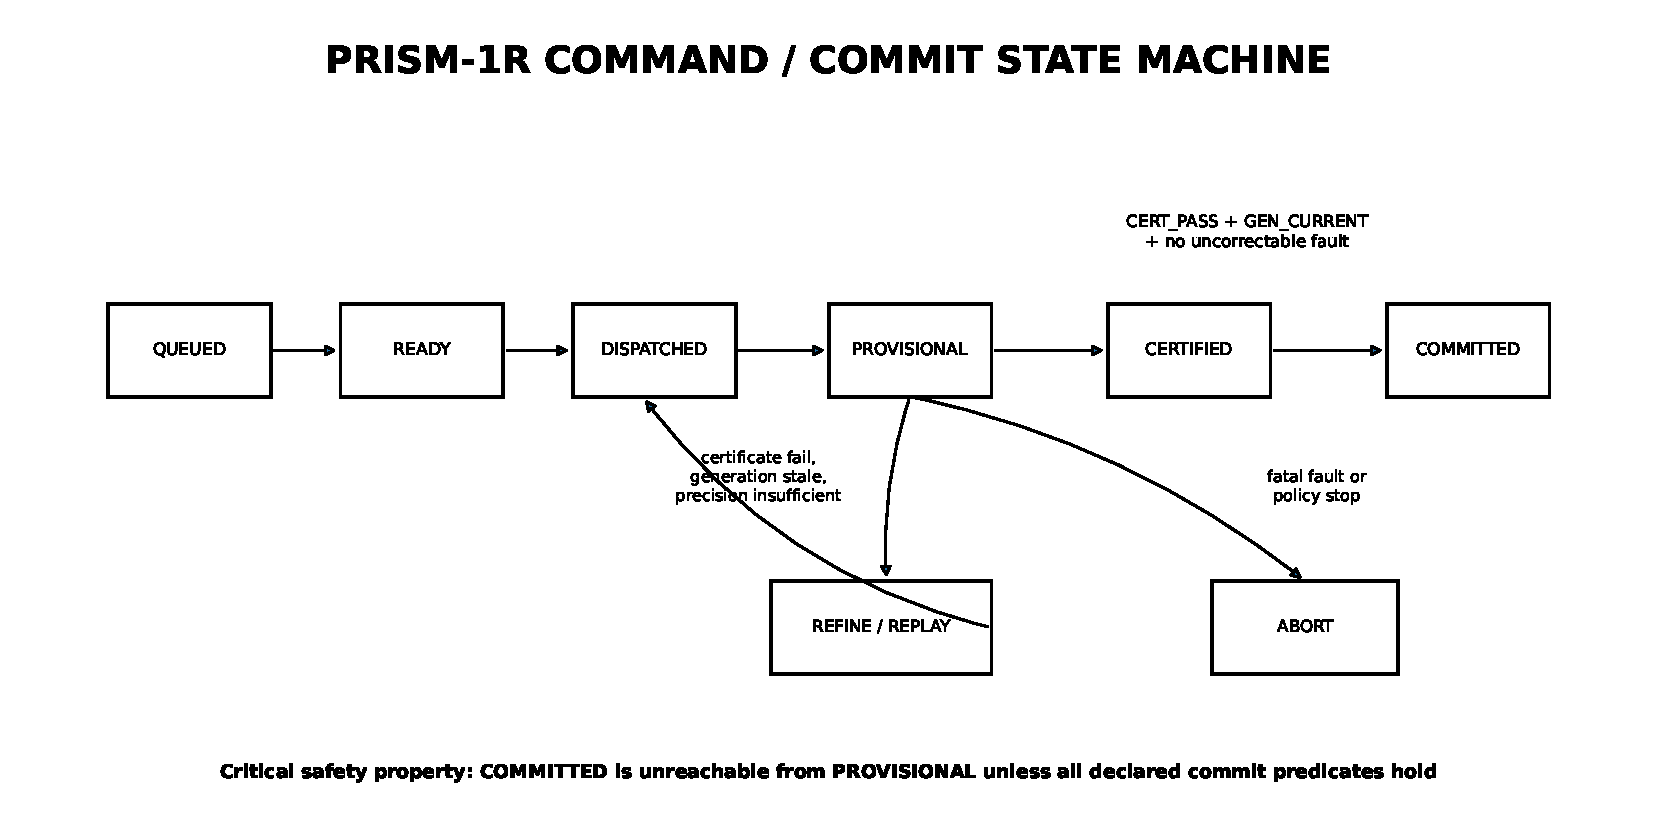
\includegraphics[width=0.96\linewidth]{../figures/04_commit_refinement_state_machine.pdf}
\caption{Command and commit state machine. The key safety property is that no direct path exists from a provisional result to committed state without the declared certificate and generation checks.}
\end{figure}

% -----------------------------------------------------------------------------
\section{Packet IR, Compiler, and Runtime Contract}

Packet IR is the stable software/hardware boundary. CUDA and PRISM backends consume the same typed graph and must preserve the same mathematical output contract.

\subsection{Planner objective}

The PRISM-1R planner should minimize a physicalized cost rather than arithmetic alone:
\[
C(G)=
\alpha F
+\beta B_{\rm HBM}
+\gamma B_{\rm SRAM}
+\delta H_{\rm NoC}
+\eta L_{\rm sync}
+\kappa C_{\rm cert}
+\rho\,\mathbb E[C_{\rm replay}].
\]

Here $F$ is arithmetic work, $B_{\rm HBM}$ and $B_{\rm SRAM}$ are bytes moved at each level, $H_{\rm NoC}$ is hop-bytes, $L_{\rm sync}$ is synchronization cost, $C_{\rm cert}$ is certificate cost, and the final term accounts for expected replay after adaptive refinement.

A decomposition is not beneficial merely because it has a structured name. The compiler must include a generic fallback leaf and negative controls.

\subsection{Software layers}

\begin{enumerate}
\item Mathematical reference kernels and conformance vectors.
\item Packet IR builder, validator, serializer, and graph visualizer.
\item Representation/resolution/placement/precision planner.
\item CUDA packet backend.
\item PRISM functional simulator.
\item PRISM cycle-aware simulator.
\item Runtime queues, allocator, residency manager, telemetry, and driver interface.
\item FPGA firmware and hardware driver.
\item ASIC firmware and package runtime.
\end{enumerate}

% -----------------------------------------------------------------------------
\section{Command and Descriptor ABI}

Use a fixed command envelope with versioned payload schemas. Opcode semantics should remain stable across CUDA emulation, simulator, FPGA, and ASIC.

\subsection{Candidate 256-bit Packet Seed Command envelope}

The following packing is a \emph{prototype ABI candidate}, not a frozen physical bit allocation. Its purpose is to prove that command identity, dependency identity, generation identity, and certificate identity fit comfortably in a compact fixed-width envelope.

\begin{table}[ht]
\centering
\caption{Candidate Packet Seed Command fields.}
\begin{tabularx}{0.96\linewidth}{p{1.45in}rX}
\toprule
\textbf{Field} & \textbf{Bits} & \textbf{Role}\\
\midrule
opcode & 8 & operation family\\
flags & 8 & deterministic mode, replay policy, privilege and compact modifiers\\
ABI version & 8 & command compatibility guard\\
format & 8 & arithmetic / payload format class\\
packet ID & 32 & primary packet identity\\
source descriptor & 32 & source descriptor-table index or handle\\
destination descriptor & 32 & destination descriptor-table index or handle\\
dependency token & 24 & readiness / wakeup dependency\\
generation & 24 & consumed packet-family generation\\
certificate ID & 24 & acceptance-rule record\\
payload or immediate & 56 & compact immediate, pointer fragment, shape class, or opcode-specific payload\\
\midrule
Total & 256 & fixed command envelope\\
\bottomrule
\end{tabularx}
\end{table}

\begin{figure}[ht]
\centering
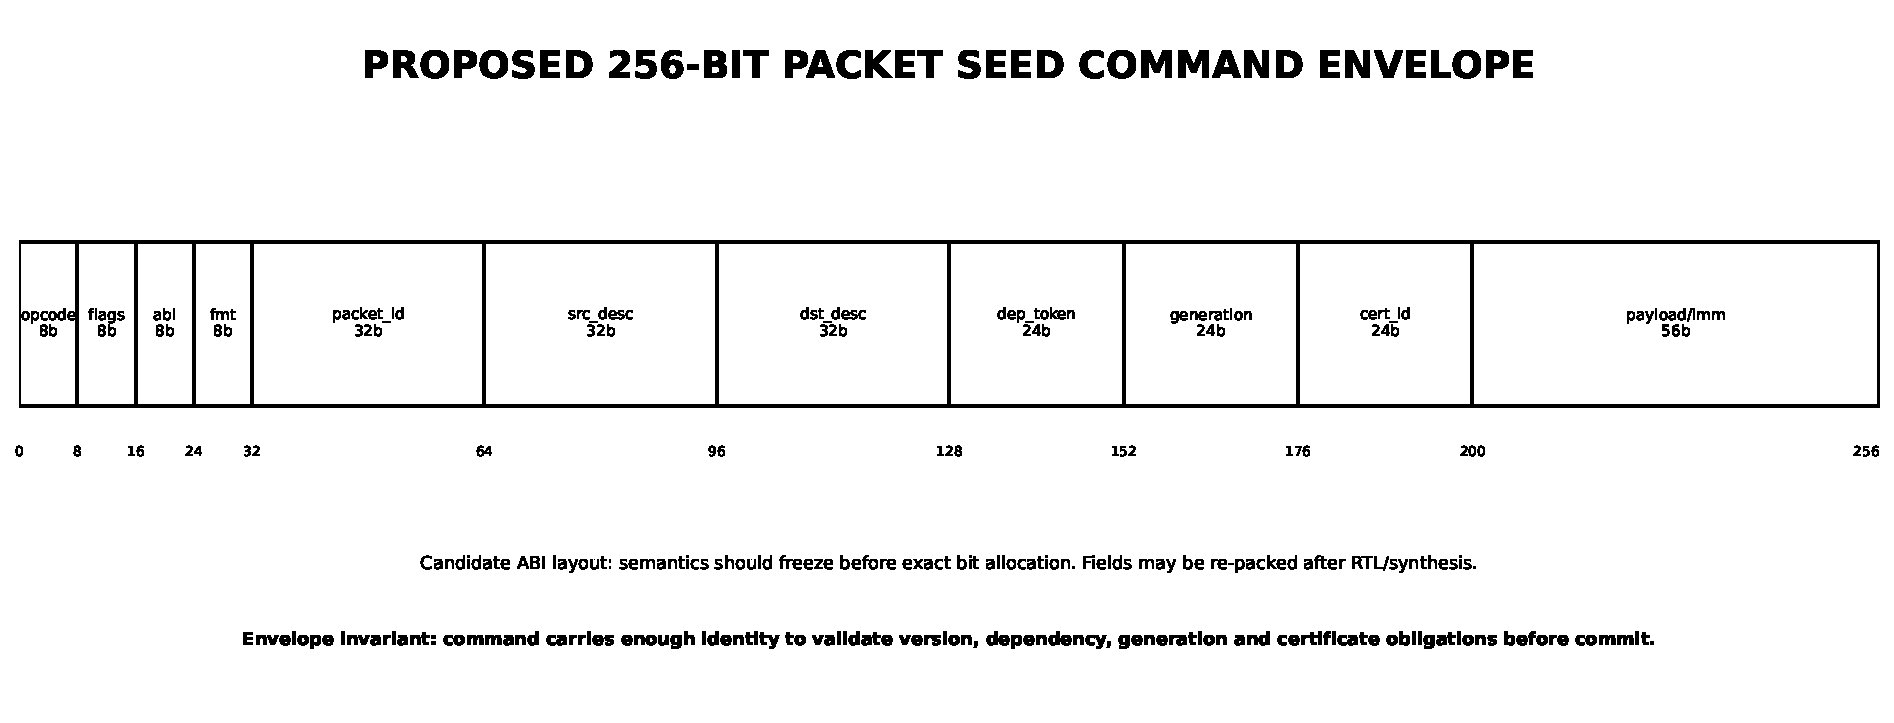
\includegraphics[width=0.98\linewidth]{../figures/06_command_envelope.pdf}
\caption{Proposed 256-bit command envelope. Semantic fields should freeze before the final bit positions do.}
\end{figure}

\subsection{Candidate packet descriptor packing}

A first 256-bit packet descriptor can carry the following information without external expansion for common cases:

\begin{center}
\begin{tabular}{lr}
\toprule
packet ID / parent ID & $32+32$ bits\\
atlas ID / selector ID & $24+24$ bits\\
shape dimensions 0 and 1 & $16+16$ bits\\
location or compact pointer & 32 bits\\
precision / error-budget class & $8+8$ bits\\
generation & 24 bits\\
flags & 16 bits\\
reserved / extension class & 24 bits\\
\midrule
Total & 256 bits\\
\bottomrule
\end{tabular}
\end{center}

Larger ranks, higher-dimensional shapes, or wide pointers use extension records rather than silently changing the base record interpretation.

\subsection{Minimum descriptor classes}

\begin{itemize}
\item packet descriptor;
\item transfer-edge descriptor;
\item atlas descriptor;
\item refinement-family descriptor;
\item precision / sensitivity / error-budget record;
\item dependency and completion token;
\item generation record;
\item residency record;
\item completion record;
\item certificate record.
\end{itemize}

\subsection{Minimum first-generation commands}

{\small\begin{longtable}{p{1.45in}p{5.05in}}
\toprule
\textbf{Command} & \textbf{Meaning}\\
\midrule
\endfirsthead
\toprule
\textbf{Command} & \textbf{Meaning}\\
\midrule
\endhead
\code{PSELECT} & apply a packet selector without materializing a dense projector\\
\code{PSPLIT} & replace a parent packet with a declared child family\\
\code{PCOARSEN} & reconstruct a parent from a complete child family\\
\code{POLYPHASE} & extract, permute, or interleave residue / phase channels\\
\code{WAVELET\_LIFT} & execute lifting predict/update/scale stages\\
\code{BLK\_GEMM} & execute equal-shape block transfer batches\\
\code{BDLR\_APPLY} & apply block-diagonal-plus-low-rank form without dense materialization\\
\code{HANKEL\_BUILD} & stream moment packets into a compact Hankel system\\
\code{ROOT\_PHASE} & perform small root / phase recovery sequence\\
\code{GRAPH\_REFINE} & replace one parent task with a local child graph\\
\code{RESIDUAL} & form / accumulate a declared reconstruction residual\\
\code{COMMIT} & publish a provisional result after certificate and generation checks\\
\code{GENERIC} & execute a non-specialized compatibility leaf\\
\bottomrule
\end{longtable}

% -----------------------------------------------------------------------------
\section{Deployment Ladder and Exit Gates}

\begin{figure}[ht]
\centering
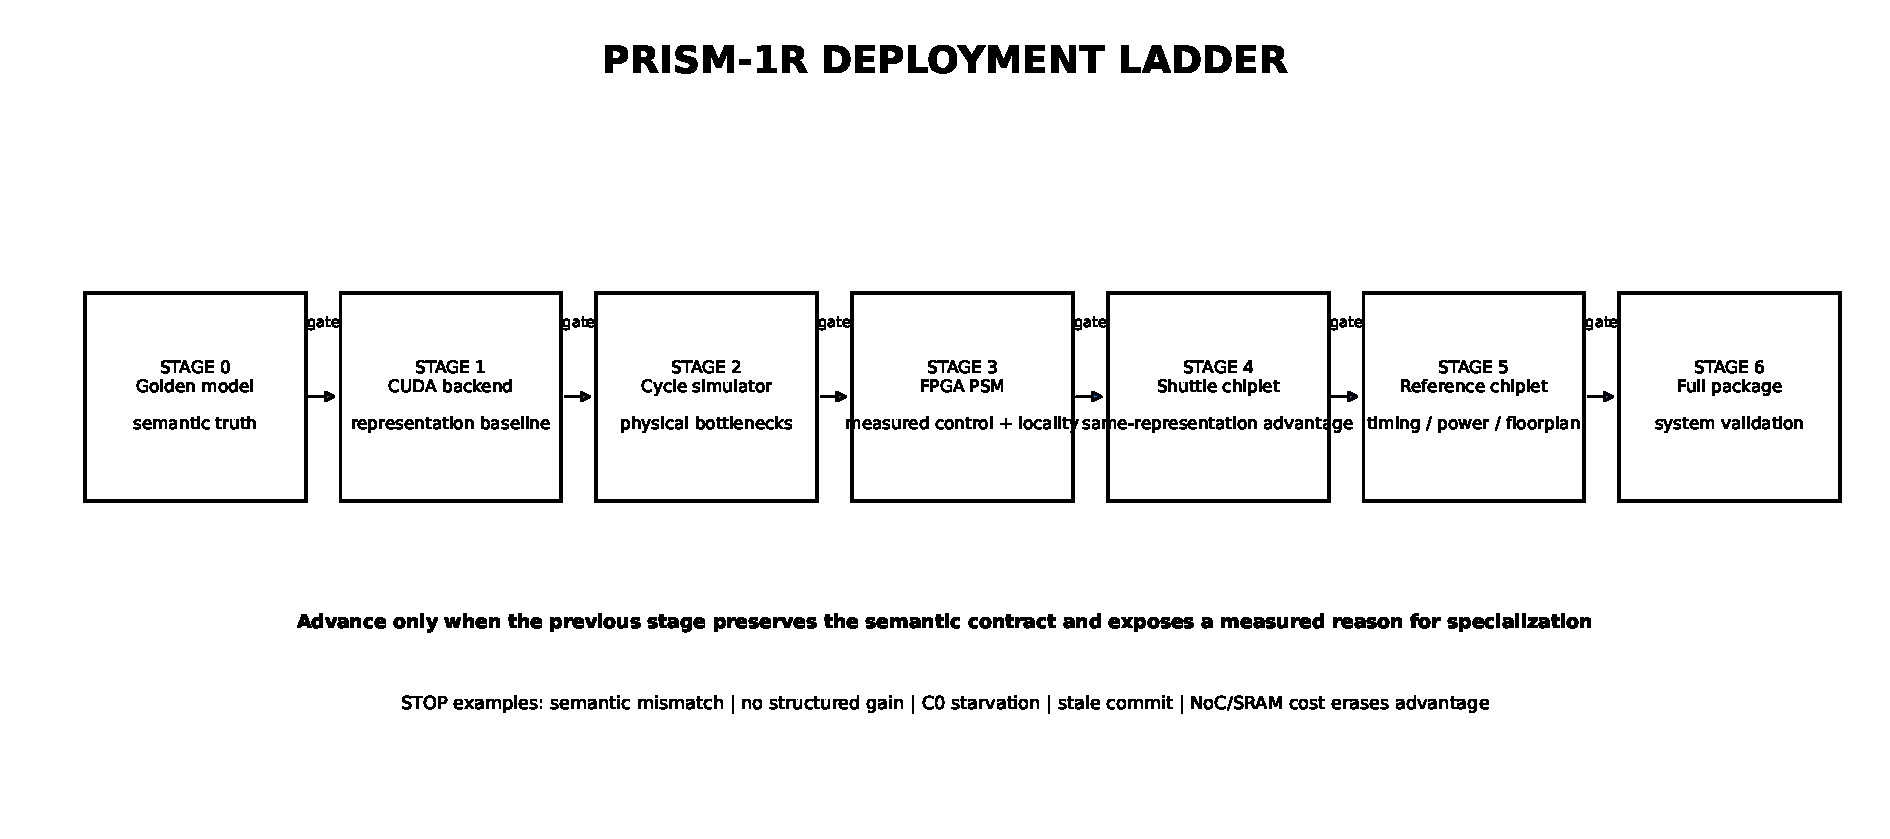
\includegraphics[width=0.98\linewidth]{../figures/05_deployment_ladder.pdf}
\caption{Deployment ladder. Each stage exists to remove a different class of uncertainty before more expensive hardware is attempted.}
\end{figure}

No stage advances because later hardware is attractive. It advances only when the preceding stage proves the contracts and exposes a measurable reason to continue.

{\footnotesize\begin{longtable}{p{0.32in}p{0.92in}p{1.50in}p{1.88in}p{1.23in}}
\toprule
\textbf{Stage} & \textbf{Artifact} & \textbf{Purpose} & \textbf{Exit gate} & \textbf{Stop condition}\\
\midrule
\endfirsthead
\toprule
\textbf{Stage} & \textbf{Artifact} & \textbf{Purpose} & \textbf{Exit gate} & \textbf{Stop condition}\\
\midrule
\endhead
0 & Golden model & Freeze Packet IR semantics, reference kernels, certificates, replay, deterministic traces & All reference vectors pass; no ambiguous descriptor semantics & semantic mismatch\\
1 & CUDA packet backend & Prove the calculus runs on existing hardware and establish realistic baselines & Structured routes reduce bytes, work, or end-to-end cost on declared workload classes & only naming structure, no real reduction\\
2 & Cycle simulator & Model banks, queueing, NoC, contention, solver / transform occupancy, replay & No deadlock; calibrated bottleneck model; C0 forward progress under C2 saturation & model cannot reproduce measured microbenchmarks\\
3 & FPGA PSM & Measure command path, DMA, bank conflicts, generation guard, certificates, local replay & ABI conformance and measured execution of representative packet graphs & semantics change to fit FPGA\\
4 & Shuttle chiplet & Measure locality, hop-bytes, factor residency, transform-to-solver handoff & Stable same-representation advantage over optimized packet GPU for target classes & NoC / SRAM cost erases advantage\\
5 & Reference chiplet & Close chiplet timing, power, SRAM macros, network widths, DVFS & Full chiplet passes functional, timing, power and reliability gates & physical closure requires removing core semantics\\
6 & Full package & Validate multi-chiplet placement, HBM, package fabric, thermals and system software & Package-level performance and reliability goals achieved & package overhead dominates structured gain\\
\bottomrule
\end{longtable}

% -----------------------------------------------------------------------------
\section{Stage 0: Golden Model}

The golden model is the authoritative semantic implementation. It must be deliberately slow if necessary. Its purpose is correctness and traceability.

Required outputs for every graph execution:

\begin{itemize}
\item canonical Packet IR graph hash;
\item packet and transfer descriptors after validation;
\item chosen representation and resolution;
\item expected output contract;
\item arithmetic count and byte-count estimates;
\item dependency and generation trace;
\item provisional outputs;
\item certificate inputs and acceptance result;
\item replay/refinement events;
\item final committed outputs.
\end{itemize}

The golden model should be the source of conformance vectors used by every later backend.

% -----------------------------------------------------------------------------
\section{Stage 1: CUDA Packet Backend}

The CUDA stage establishes the most important baseline: how far the representation itself can go before custom hardware contributes anything.

Each experiment should separate:
\[
S_{\rm representation},\quad S_{\rm backend},\quad S_{\rm architecture},\quad S_{\rm amortized}.
\]

Never report a combined ratio without preserving those components.

Measure grouped block kernels, asynchronous transfers, factor residency, transform libraries, sparse kernels, Woodbury paths, packetwise mixed precision, graph replay, and negative controls.

\statusbox{CUDA gate.}{Custom hardware is justified only for bottlenecks that remain after the packet representation is already implemented competently on an existing GPU.}

% -----------------------------------------------------------------------------
\section{Stage 2: Cycle-Aware Simulator}

The simulator must add physical constraints absent from the golden model:

\begin{itemize}
\item 16-bank scratchpad conflicts and queueing;
\item execution-group issue / completion timing;
\item transform and solver contention;
\item C0-C3 network arbitration;
\item multicast and tree reductions;
\item shared-SRAM residency and eviction;
\item dependency wakeups;
\item certificate latency;
\item generation mismatch and local replay;
\item HBM request scheduling;
\item thermal / DVFS hooks for later calibration.
\end{itemize}

The simulator should produce cycle-by-cycle counters and a summarized plan report. Do not silently hide bank conflicts or network queues inside an ``effective latency'' constant.

% -----------------------------------------------------------------------------
\section{Stage 3: FPGA PSM Blueprint}

The first FPGA target implements one logical PSM. Resource scaling is permitted, semantic scaling is not.

\subsection{Required blocks}

\begin{itemize}
\item command queue and descriptor fetch;
\item dependency + generation scoreboard;
\item 16-bank or proportionally banked BRAM/URAM scratchpad;
\item four logical execution groups or time-multiplexed equivalents;
\item projector/polyphase DMA path;
\item one transform path;
\item one small-solver path;
\item residual / certificate accumulator;
\item commit / replay controller;
\item performance-counter block;
\item fault injection for descriptor, generation, and certificate errors.
\end{itemize}

\subsection{FPGA acceptance tests}

\begin{enumerate}
\item Execute a block-diagonal workload without forming a dense matrix.
\item Execute BDLR apply with resident factors.
\item Execute a transform $\rightarrow$ small solve $\rightarrow$ reconstruction chain without host round-trip.
\item Trigger a certificate failure and verify local replay.
\item Trigger a generation change while work is provisional and prove stale commit is impossible.
\item Saturate payload traffic and demonstrate forward progress of C0 commit/dependency traffic.
\item Compare all committed outputs with golden-model vectors.
\end{enumerate}

% -----------------------------------------------------------------------------
\section{Stages 4-6: ASIC Development Path}

\subsection{Stage 4: shuttle chiplet}

Use 4-8 PSMs and at least two quadrants. The key measurements are not dense FLOP/s. Measure:

\begin{itemize}
\item local versus remote packet access;
\item hop-byte distribution;
\item factor reuse per load;
\item transform-to-solver handoff latency;
\item solver occupancy;
\item refinement invalidation radius;
\item certificate bandwidth;
\item energy per committed output.
\end{itemize}

\subsection{Stage 5: reference chiplet}

Scale to 16 PSMs and four quadrants. Freeze SRAM macro organization, final physical NoC width, clock domains, DVFS, and floorplan only after evidence from synthesis and the shuttle-scale measurements.

\subsection{Stage 6: full package}

Integrate four compute chiplets, I/O/control die, HBM, UCIe-class package links, host I/O, system firmware, telemetry, fault containment, and thermal control. The full package is a final integration stage, not the first place to discover whether packet locality works.

% -----------------------------------------------------------------------------
\section{Verification and Signoff Matrix}

{\small\begin{longtable}{p{0.82in}p{2.00in}p{1.67in}p{1.65in}}
\toprule
\textbf{Domain} & \textbf{Obligation} & \textbf{Primary method} & \textbf{Pass condition}\\
\midrule
\endfirsthead
\toprule
\textbf{Domain} & \textbf{Obligation} & \textbf{Primary method} & \textbf{Pass condition}\\
\midrule
\endhead
Semantic & reconstruction, transform/synthesis identity, output contracts & golden model + property tests & no semantic mismatch\\
Control & dependency tokens, generation invalidation, replay boundary & formal assertions + randomized traces & no stale commit, no deadlock\\
Arithmetic & mixed precision, exact modes, rank/phase decisions & bit-accurate models & declared certificate bound satisfied\\
Memory & bank conflicts, allocation, ECC/parity, double buffering & cycle sim + FPGA counters & stress targets met\\
NoC & traffic classes, multicast, reduction, congestion & adversarial traffic tests & C0 forward progress, no protocol deadlock\\
Compiler & representation/resolution/placement decisions & differential testing on small graphs & plan never changes semantics\\
Reliability & malformed commands, corrupted descriptors, replay storms & fault injection & deterministic containment and reporting\\
Physical & timing, power, thermal, IR drop, CDC/reset & EDA signoff & all process/package limits satisfied\\
\bottomrule
\end{longtable}

% -----------------------------------------------------------------------------
\section{Benchmark Suite and Required Metrics}

Every benchmark report should expose at least the following quantities.

\begin{table}[h]
\centering
\begin{tabularx}{0.96\linewidth}{p{1.6in}X}
\toprule
\textbf{Metric} & \textbf{Definition / purpose}\\
\midrule
Bytes eliminated & explicit-array route bytes divided by packet-route bytes\\
Work eliminated & dense/reference arithmetic divided by executed arithmetic\\
Packet occupancy & useful execution-group cycles divided by available cycles\\
Residency reuse & number of factor/atlas uses per memory load\\
NoC cost & hop-bytes and utilization by C0-C3 traffic class\\
Refinement locality & remote state invalidated per local refinement event\\
Certificate overhead & certificate cycles and bytes divided by total execution\\
Replay cost & useful work discarded or repeated after refinement\\
Energy & joules per committed output\\
Fallback quality & fraction of negative controls correctly routed away from specialization\\
\bottomrule
\end{tabularx}
\end{table}

Representative workload families should include structured linear operators, BDLR, regular block sparse graphs, transform-domain operators, unknown-edge reconstruction, small-solver-heavy chains, packet Bayesian portfolios, exact modular/residue workloads, and deliberately unstructured negative controls.

% -----------------------------------------------------------------------------
\section{Deployment Runbook}

\begin{enumerate}
\item \textbf{Build.} Compile the reference kernels, Packet IR tools, planner, CUDA backend, simulator, firmware, driver, and target image from one tagged release.
\item \textbf{Conformance.} Run descriptor schema tests and golden vectors before allowing hardware execution.
\item \textbf{Discover.} Query target capabilities: ABI version, PSM count, bank topology, formats, transform/solver inventory, link width, and exact-mode support.
\item \textbf{Preload.} Place immutable hot atlases and factors where reuse is expected.
\item \textbf{Plan.} Compile representation, resolution, placement, precision, and certificate plan. Emit a human-readable plan report.
\item \textbf{Execute.} Submit versioned command buffers and record queue, bank, NoC, execution, certificate, and replay telemetry.
\item \textbf{Validate.} Compare committed outputs against exact expectations or reference tolerances. Never consume provisional outputs.
\item \textbf{Profile.} Attribute bottlenecks separately to HBM, scratchpad banks, NoC, transforms, solvers, certificates, or replay.
\item \textbf{Promote.} Make a specialized route default only after repeatable wins and passing negative controls.
\item \textbf{Regress.} Re-run the canonical benchmark and fault-injection suites for every compiler, firmware, RTL, or physical-parameter change.
\end{enumerate}

% -----------------------------------------------------------------------------
\section{Failure Policy}

The deployment process should fail visibly rather than convert uncertainty into optimistic defaults.

\begin{table}[h]
\centering
\begin{tabularx}{0.96\linewidth}{p{1.8in}X}
\toprule
\textbf{Failure} & \textbf{Required response}\\
\midrule
Unknown descriptor version & reject before execution\\
Uncorrectable descriptor corruption & abort affected command and invalidate dependent provisional work\\
Generation mismatch & prevent commit; replay smallest declared region\\
Certificate failure & refine, increase precision, choose alternate representation, or abort according to policy\\
C0 starvation & architecture bug; test must fail\\
Planner chooses unsupported feature & lower to legal fallback or reject; never reinterpret silently\\
Negative control forced into specialization & compiler quality failure\\
Backend disagrees with golden semantics & release-blocking error\\
Timing/power closure requires semantic weakening & stop physical implementation and redesign rather than changing the contract silently\\
\bottomrule
\end{tabularx}
\end{table}

% -----------------------------------------------------------------------------
\section{RTL Partition and Interface Blueprint}

The first RTL release should be deliberately narrow. The objective is to make the safety and scheduling boundaries executable before attempting high-throughput kernels.

\begin{lstlisting}
rtl/
  include/
    prism_types_pkg.sv
  core/
    prism_command_frontend.sv
    prism_descriptor_cache.sv
    prism_dependency_scoreboard.sv
    prism_generation_guard.sv
    prism_representation_router.sv
    prism_resolution_controller.sv
    prism_scratchpad_banks.sv
    prism_eg_cluster.sv
    prism_transform_port.sv
    prism_solver_port.sv
    prism_certificate_accumulator.sv
    prism_commit_controller.sv
    prism_psm_top.sv
  noc/
    prism_control_router.sv
    prism_packet_router.sv
    prism_multicast_unit.sv
    prism_reduction_unit.sv
  tb/
    tb_commit_semantics.sv
    tb_generation_race.sv
    tb_c0_forward_progress.sv
    tb_local_replay.sv
\end{lstlisting}

The accompanying handoff package includes boundary skeletons for the generation guard, commit controller, a PSM top-level shell, and a smoke-test bench. These are semantic scaffolds, not production RTL.

\subsection{Recommended ready/valid discipline}

All command, descriptor, and data interfaces should use explicit backpressure. A sender may not infer acceptance from elapsed cycles. For every channel:
\[
\texttt{transfer}=\texttt{valid}\land\texttt{ready}.
\]

Metadata and payload channels should carry a transaction identity sufficient to detect mismatched completion records in simulation and debug builds.

% -----------------------------------------------------------------------------
\section{PSM Pipeline and Scheduling Contract}

A practical first implementation can expose the following logical pipeline. Physical retiming may alter cycle counts but must preserve the boundaries.

\begin{enumerate}
\item \textbf{Fetch}: read fixed-width command envelope.
\item \textbf{Validate}: check ABI, opcode, descriptor bounds, privilege, and basic format legality.
\item \textbf{Resolve}: fetch packet, transfer, generation, and certificate descriptors.
\item \textbf{Ready}: dependency scoreboard confirms all required inputs are eligible.
\item \textbf{Reserve}: allocate scratchpad destination, execution route, and completion entry.
\item \textbf{Execute}: issue transformation or resolution work to the chosen engine.
\item \textbf{Provisional completion}: capture output identity, bytes, cycles, residual summary, and consumed generation.
\item \textbf{Commit resolution}: certificate + generation + fault + dependency predicate chooses commit, replay, or abort.
\end{enumerate}

The scheduler may overlap commands aggressively, but it may not elide stages 3, 7, or 8. Those stages carry the semantic obligations that distinguish completion from commitment.

\subsection{Scoreboard entries}

At minimum, an in-flight entry should retain command ID, packet ID, consumed generation, dependency token, destination reservation, certificate ID, replay-region ID, engine assignment, and current state. Debug builds should additionally retain timestamps for every state transition.

% -----------------------------------------------------------------------------
\section{Scratchpad Bank Contract}

The 16 physical banks should be exposed to the allocator through a bank-mapping function rather than a fixed contiguous modulo mapping. Polyphase and strided packet accesses can otherwise create systematic conflict patterns.

A prototype mapping may use a configurable XOR swizzle,
\[
\operatorname{bank}(w)=
\bigl(w_{3:0}\oplus w_{7:4}\oplus h(P)\bigr)\bmod 16,
\]
where $w$ is the local word index and $h(P)$ is a four-bit packet/phase hash. This is an implementation policy, not part of the mathematical contract, and should be replaced if FPGA counters show worse behavior for target transforms.

Bank arbitration must report conflicts to performance counters. The simulator and FPGA must agree on the definition of a bank-conflict cycle before architectural performance claims are made.

% -----------------------------------------------------------------------------
\section{Formal Safety Invariants}

The following properties should be encoded as assertions in the RTL and independently checked in the reference model.

\begin{description}[leftmargin=1.35in,style=nextline]
\item[I1: stale-commit exclusion] If the consumed generation differs from the current generation, \texttt{commit} is false.
\item[I2: certificate gating] If a required certificate is unfinished or failed, \texttt{commit} is false.
\item[I3: fault containment] An uncorrectable protected-state fault cannot produce a committed result.
\item[I4: dependency validity] A completion token cannot release downstream committed work before the producing command commits.
\item[I5: replay locality] A retryable failure invalidates only the declared replay region and its dependent provisional descendants.
\item[I6: control forward progress] Under finite injection and a responsive destination, C0 traffic cannot be permanently starved by C2/C3 traffic.
\item[I7: deterministic mode] When deterministic mode is requested, reduction topology, rounding mode, and replay decisions are reproducible from the same command and state trace.
\item[I8: backend semantic equivalence] CUDA, golden-model, FPGA, and ASIC executions of the same legal Packet IR program satisfy the same declared output contract.
\end{description}

For I1 the hardware-level implication is simply
\[
(g_{\rm consumed}\neq g_{\rm current})\Rightarrow \neg\texttt{commit}.
\]
The implementation package includes a minimal executable reference test for this invariant.

% -----------------------------------------------------------------------------
\section{Boot, Discovery, and Runtime Bring-Up}

A target should not accept general packet programs immediately after reset. Recommended bring-up order:

\begin{enumerate}
\item reset all PSMs, queues, routers, certificate accumulators, and generation tables;
\item verify ROM / firmware image and ABI compatibility;
\item scrub or initialize descriptor SRAM and protected control memories;
\item enumerate PSM, transform, solver, exact-arithmetic, SRAM-bank, HBM, and link capabilities;
\item run a local self-test for scratchpad banks, command queue, generation guard, and commit controller;
\item run a cross-quadrant C0/C2 traffic smoke test;
\item publish the capability block to the host runtime;
\item accept only Packet IR plans whose required feature set is a subset of the discovered capabilities.
\end{enumerate}

A failed generation-guard or commit-controller self-test is a hard device-disable condition. A failed transform or solver self-test may permit a degraded capability profile if the runtime can route those operations elsewhere without changing semantics.

% -----------------------------------------------------------------------------
\section{Telemetry and Performance-Counter Minimum Set}

Every PSM should expose counters sufficient to distinguish a poor mathematical plan from a poor hardware mapping. Minimum counters:

\begin{itemize}
\item commands fetched, issued, completed, committed, replayed, and aborted;
\item cycles stalled on dependency, destination allocation, scratchpad banks, NoC, transform, solver, certificate, and HBM;
\item scratchpad bytes read/written by P/F/M/R logical class;
\item bank-conflict cycles by bank and access class;
\item NoC flits or bytes by C0-C3 class and hop count;
\item factor / atlas reuse count;
\item generation mismatch count;
\item certificate failure count by reason;
\item replayed cycles and bytes;
\item deterministic-mode invocations;
\item corrected and uncorrectable protected-state errors.
\end{itemize}

The planner calibration loop should consume these counters directly rather than tuning against wall-clock time alone.

% -----------------------------------------------------------------------------
\section{Implementation Handoff Package}

The v0.2 package accompanies this PDF with:

\begin{itemize}
\item Python-generated PDF, SVG, and PNG engineering blueprints;
\item the Python figure generator;
\item SystemVerilog semantic boundary skeletons for generation and commit logic;
\item a minimal Python semantic reference model;
\item executable smoke tests for valid commit, stale generation replay, and fatal-fault abort;
\item a manifest and status boundary distinguishing implemented scaffolding from future production RTL.
\end{itemize}

The supplied Python semantic tests pass in the build environment. No SystemVerilog compiler was available in that environment, so the RTL skeleton is \emph{not} claimed to have passed HDL compilation or synthesis.

% -----------------------------------------------------------------------------
\section{Architecture Freeze Checklist}

A PRISM-1R implementation is ready to enter production RTL only when all items below are checked.

\begin{enumerate}[label=$\square$]
\item Packet / transfer / atlas / refinement / generation descriptor schemas are versioned.
\item Packet IR canonical serialization is stable.
\item Output contracts are explicit and tested.
\item Commit and replay state machines are formally specified.
\item Generation invalidation rules are formally specified.
\item Minimum C0-C3 traffic guarantees are specified.
\item Scratchpad allocator contract and bank-conflict behavior are specified.
\item Supported arithmetic formats and rounding rules are fixed.
\item Exact arithmetic obligations are bounded and specified.
\item Transform and small-solver minimum operation set is fixed.
\item CUDA and PRISM conformance vectors pass.
\item Golden model is reproducible from a tagged release.
\item Cycle simulator reports all modeled queues and conflicts.
\item FPGA prototype demonstrates stale-commit prevention.
\item FPGA prototype demonstrates certificate-triggered local replay.
\item Negative controls route correctly.
\item Benchmark reports separate representation, backend, architecture, and amortized effects.
\item Fault-injection suite passes.
\end{enumerate}

% -----------------------------------------------------------------------------
\section{First 30 Engineering Tasks}

{\small\begin{longtable}{r p{6.15in}}
\toprule
\textbf{No.} & \textbf{Task}\\
\midrule
\endfirsthead
\toprule
\textbf{No.} & \textbf{Task}\\
\midrule
\endhead
1 & Freeze Packet IR schema version 1.\\
2 & Freeze packet, transfer, atlas, refinement, generation, and certificate descriptors.\\
3 & Implement canonical binary/JSON serialization and schema validator.\\
4 & Build deterministic golden Packet IR interpreter.\\
5 & Define canonical execution trace format.\\
6 & Implement generation guard in golden model.\\
7 & Implement certificate state machine in golden model.\\
8 & Implement local replay region semantics.\\
9 & Port representative block-diagonal and BDLR graphs to canonical Packet IR.\\
10 & Port transform-to-small-solver reconstruction chain.\\
11 & Implement CUDA grouped block backend.\\
12 & Implement CUDA factor-resident BDLR backend.\\
13 & Implement CUDA transform/solver chain with graph replay.\\
14 & Add structured and unstructured negative controls.\\
15 & Define benchmark result schema separating gain types.\\
16 & Implement PSM functional simulator.\\
17 & Add 16-bank scratchpad timing model.\\
18 & Add C0-C3 NoC queue model.\\
19 & Add quadrant placement and hop-byte accounting.\\
20 & Add transform/solver occupancy model.\\
21 & Add hierarchical certificate timing model.\\
22 & Add replay-cost estimator.\\
23 & Implement joint representation/resolution/placement cost planner.\\
24 & Write SystemVerilog command and descriptor interfaces.\\
25 & Implement FPGA scoreboard and generation guard.\\
26 & Implement FPGA scratchpad bank controller.\\
27 & Implement FPGA certificate/commit path.\\
28 & Implement fault injection and stale-generation testbench.\\
29 & Run first end-to-end FPGA conformance workload.\\
30 & Freeze shuttle-chiplet experiment matrix from measured FPGA bottlenecks.\\
\bottomrule
\end{longtable}

% -----------------------------------------------------------------------------
\section{Final Deployment Rule}

The deployment program should preserve one strict ordering:
\[
\boxed{
\text{mathematical contract}
\rightarrow
\text{software proof of execution}
\rightarrow
\text{measured bottleneck}
\rightarrow
\text{hardware specialization}.
}
\]

PRISM-1R is justified only where the representation has already removed unnecessary work and where dedicated hardware measurably improves the remaining structured computation.

The target machine is therefore not a GPU with extra packet opcodes. It is a processor in which representation, resolution, locality, uncertainty, and commit state are all architectural information.

\vfill
\begin{center}
\rule{0.8\linewidth}{0.5pt}\\[0.08in]
\small End of PRISM-1R Implementation and Deployment Blueprint v0.2
\end{center}

\end{document}
